\documentclass[xcolor=table]{beamer}

\mode<presentation>
{
  \usetheme{Madrid}      % or try Darmstadt, Madrid, Warsaw, ...
  \usecolortheme{beaver} % or try albatross, beaver, crane, ...
  \usefonttheme{professionalfonts}
  \setbeamertemplate{navigation symbols}{}
} 

\usepackage[utf8]{inputenc}
\usepackage[english]{babel}
\usepackage{tikz}
\usepackage{pgfplots}
\graphicspath{ {images/} }
\pgfplotsset{compat=1.14}


\title[Analysis of 3 voting systems]{Software implementations and analysis of three voting systems}
\author{Adrian Salamon}
\institute[Kungsholmens gymn.]{Kungsholmens gymnasium}
\date{\today}

\begin{document}

\begin{frame}
  \titlepage
\end{frame}

\section{Introduction}
\begin{frame}{Introduction}
\begin{itemize}
    \item What is a voting system?
    \item Have been interested in voting systems and wanted to test them
    \item Testing 3 methods
    \begin{itemize}
        \item First-past-the-post (FPTP)
        \item Single Transferable Vote (STV)
        \item Schulze method
    \end{itemize}
    \item Everything is done by programming
\end{itemize}
    
\end{frame}

\section{Voting systems}
\subsection{First-past-the-post}
\begin{frame}{First-past-the-post (FPTP)}
\begin{itemize}
    \item Simple majority system
    \item ``Most votes win'' and ``One person, one vote''
    \item Used widely in the Anglo-Saxon world
\end{itemize}
\centering
Example: Elect 2 from this sample:
\begin{overprint}
    \onslide<1> 
\begin{figure}[H]
	\centering
	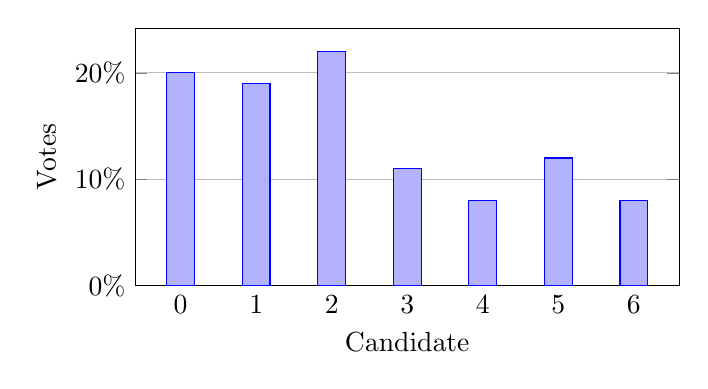
\begin{tikzpicture}
		\begin{axis}[
			ybar stacked,
			width = 0.7\textwidth,
			height = 0.4\textwidth,
			legend style={at={(0.5,-0.25)},
			anchor=north,legend columns=-1},
      x tick style = transparent,
			ylabel = {Votes},
			xlabel = {Candidate},
			ymajorgrids = true,
      ymin = 0,
			yticklabel={\pgfmathprintnumber\tick\%}
      ]
			\addplot coordinates
			{(0, 20)(1, 19)(2, 22)(3, 11)(4, 8)(5, 12)(6, 8)};
		\end{axis}
	\end{tikzpicture}
\end{figure}
    \onslide<2>
\begin{figure}[H]
	\centering
	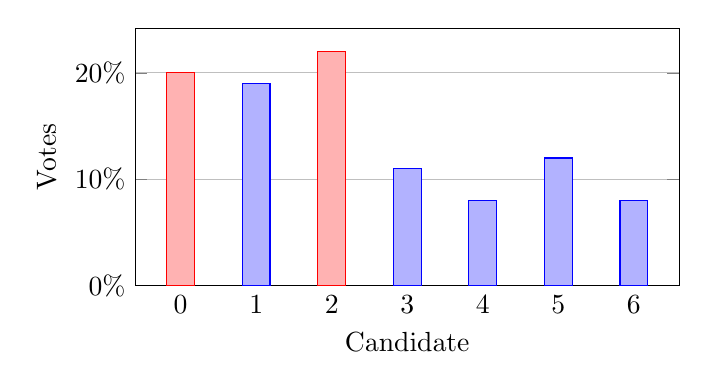
\begin{tikzpicture}
		\begin{axis}[
			ybar stacked,
			width = 0.7\textwidth,
			height = 0.4\textwidth,
			legend style={at={(0.5,-0.25)},
			anchor=north,legend columns=-1},
      x tick style = transparent,
			ylabel = {Votes},
			xlabel = {Candidate},
			ymajorgrids = true,
      ymin = 0,
			yticklabel={\pgfmathprintnumber\tick\%}
      ]
			\addplot coordinates
			{(0, 0)(1, 19)(2, 0)(3, 11)(4, 8)(5, 12)(6, 8)};
            \addplot coordinates
			{(0, 20)(1, 0)(2, 22)(3, 0)(4, 0)(5, 0)(6, 0)};
		\end{axis}
	\end{tikzpicture}
\end{figure}
\end{overprint}

    
\end{frame}

\subsection{Single Transferable Vote}
\begin{frame}{Single Transferable Vote (STV)}
\begin{itemize}
    \item Uses ballots where voters rank candidates in order
    \item Uses this data to transfer votes between candidates within a ballot
    \item A quota/threshold is defined
    \item If a candidate exceeds threshold, excess votes are transferred
    \item If no candidate reaches threshold, the candidate with fewest votes gets eliminated and his/her votes are transferred
\end{itemize}
\begin{figure}
	\centering
	\includegraphics[height=80px]{ballot}
\label{fig:stv ballot}
\end{figure}
\end{frame}
\subsection{Schulze method}
\begin{frame}{Schulze method}
\begin{itemize}
    \item Is a \textit{Condorcet method}
    \item Compares all candidates in pairwise comparisons
    \item If any candidate wins every pairwise comparison, he/she is the Condorcet winner
    \item If there is no such candidate, path strengths are calculated and compared
\end{itemize}
\begin{table}
\centering
\begin{tabular}{l|c|c|c|c|c|}
\cline{2-6}
 & \multicolumn{1}{l|}{A} & \multicolumn{1}{l|}{B} & \multicolumn{1}{l|}{C} & \multicolumn{1}{l|}{D} & \multicolumn{1}{l|}{E} \\ \hline
\multicolumn{1}{|l|}{A} & \cellcolor[HTML]{9B9B9B} & \cellcolor[HTML]{FFDDDD}17 & \cellcolor[HTML]{FFDDDD}14 & \cellcolor[HTML]{DDFFDD}35 & \cellcolor[HTML]{DDFFDD}30 \\ \hline
\multicolumn{1}{|l|}{B} & \cellcolor[HTML]{DDFFDD}33 & \cellcolor[HTML]{9B9B9B} & \cellcolor[HTML]{FFDDDD}24 & \cellcolor[HTML]{DDFFDD}47 & \cellcolor[HTML]{DDFFDD}36 \\ \hline
\multicolumn{1}{|l|}{C} & \cellcolor[HTML]{DDFFDD}36 & \cellcolor[HTML]{DDFFDD}26 & \cellcolor[HTML]{9B9B9B} & \cellcolor[HTML]{DDFFDD}40 & \cellcolor[HTML]{DDFFDD}42 \\ \hline
\multicolumn{1}{|l|}{D} & \cellcolor[HTML]{FFDDDD}15 & \cellcolor[HTML]{FFDDDD}3 & \cellcolor[HTML]{FFDDDD}10 & \cellcolor[HTML]{9B9B9B} & \cellcolor[HTML]{FFDDDD}18 \\ \hline
\multicolumn{1}{|l|}{E} & \cellcolor[HTML]{FFDDDD}20 & \cellcolor[HTML]{FFDDDD}14 & \cellcolor[HTML]{FFDDDD}8 & \cellcolor[HTML]{DDFFDD}32 & \cellcolor[HTML]{9B9B9B} \\ \hline
\end{tabular}
\end{table}
\end{frame}

\section{Methodology}
\subsection{Vote generation}
\begin{frame}{Generation of vote data}
\begin{itemize}
    \item No publicly available election data was found
    \item A program to create elections was developed
    \item Better than random data
    \item Includes the concept of an ``ideology'' that split the population.
    \item The program takes a simple configuration object and generates an election result
    \item Three election scenarios were tested, each based on a different configuration object
\end{itemize}
    
\end{frame}
\subsection{Implementations}
\begin{frame}{Programming implementations}
\begin{itemize}
    \item Everything was implemented in Typescript and tested.
    \item All code is open sourced under the MIT licence and available on Github.
    \item Added 5547 thousand lines and deleted 3305 thousand lines
    \item \url{https://github.com/adriansalamon/gymnasiearbete}
\end{itemize}
\end{frame}


\section{Results and conclusions}
\subsection{Example of Results}
\begin{frame}{Example of results}
\begin{figure}[H]
	\centering
	
\begin{tikzpicture}
		\begin{axis}[
			ybar,
			width = 1\textwidth,
			height = 0.7\textheight,
			legend style={at={(0.5,-0.25)},
			anchor=north,legend columns=-1},
      x tick style = transparent,
			ylabel = {Elections won},
			xlabel = {Candidate},
			ymajorgrids = true,
			every axis plot/.append style={draw=none,fill,no markers},
      ymin = 0,
			symbolic x coords={0,1,2,3,4,5,6,7,8},
			bar width=0.25cm
      ]
			\addplot coordinates
			{(0, 973)(1, 267)(2, 1000)(3, 0)(4, 12)(5, 743)(6, 0)(7, 5)(8, 0)};
			\addplot coordinates
			{(0, 456)(1, 808)(2, 1000)(3, 0)(4, 33)(5, 703)(6, 0)(7, 0)(8, 0)};
			\addplot coordinates
			{(0, 338)(1, 160)(2, 1000)(3, 0)(4, 0)(5, 1000)(6, 0)(7, 502)(8, 0)};
			\legend{FPTP, STV, Schulze}
		\end{axis}
	\end{tikzpicture}
\end{figure}
    
\end{frame}
\subsection{Conclusions}
\begin{frame}{Conclusions}
I made 4 conclusions:
\begin{itemize}
    \item Schulze did not seem to be a proportional voting method in multi-seat elections
    \item In single-seat elections, Schulze and STV seemed to provide similar results
    \item FPTP did not seem to be a very proportional method in close elections
    \item STV seems to be the most proportional method out of the 3 tested, but is not without its flaws
\end{itemize}
\end{frame}

\subsection{Further work}
\begin{frame}{Further work}
\begin{itemize}
    \item Create more and better test data. Maybe even real election data.
    \item Test more election methods
    \item Since all code is open source, anyone can freely copy and modify it to further build on the work presented in this paper.
    \item The implementations provided in this paper can also be used for other projects such as online voting websites.
\end{itemize}
    
\end{frame}


\end{document}